\section{Von der klassischen Mechanik zur Quantenmechanik}
\begin{frame}{Klassische Dynamik von Teilchen}
\begin{figure}
\begin{tikzpicture}
\centering

%Koordinatensystem
\draw[->, thick] (0,0) to (10,0);
\node at (10.3,0) {\Large$t$};
\draw[->, thick] (0,0) to (0,6.5);
\node at (0,6.8) {\Large$q$};

%Punkte
\filldraw (2,2)   circle (2pt);
\node at (1.6,1.8) {\Large$a$};
\filldraw (8,5)   circle (2pt);
\node at (8.4,5.2) {\Large$b$};

%Trajektorie
\draw[-, thick] (2,2) to [curve through = {(3, 1.9) (3.7,3.4)  (4.5,5)}] (8,5);

\end{tikzpicture}
\caption{Trajektorie eines klassischen Punktteilchens}
\end{figure}
\end{frame}

\begin{frame}{Klassische Dynamik von Teilchen}
\begin{itemize}
	\item Trajektorien ergeben sich aus dem \textbf{Wirkungsprinzip}, das heißt die Wirkung $\mathcal{S}$, mit
	\begin{align*}
	\mathcal{S} = \int_{t_1}^{t_2} \dd t \ \mathcal{L}(q(t),\dot{q}(t)) 
	\end{align*}
	soll minimiert werden.
	\item Dazu muss die erste Variation $\delta\mathcal{S}$ verschwinden:
	\begin{align*}
		\delta \mathcal{S} = \int_{t_1}^{t_2} \dd t \left(\frac{\partial \mathcal{L}}{\partial q} \delta q + \frac{\partial \mathcal{L}}{\partial \dot{q}} \delta \dot{q}\right) \overset{!}{ = } 0
	\end{align*}
	\item Ausführen der Variation liefert \textbf{Euler-Lagrange-Gleichungen:} 
	\begin{align*}
		\frac{\dd}{\dd t}\frac{\partial \mathcal{L}}{\partial \dot{q}} - \frac{\partial \mathcal{L}}{\partial q} = 0
	\end{align*}
\end{itemize}
\end{frame}

\begin{frame}{Bisheriger Zugang zur Quantenmechanik}
\begin{itemize}
	\item Determinismus $\longrightarrow $ Wahrscheinlichkeitsaussagen
	\item Zentrale Objekte sind \textbf{Zustände} $\ket{\psi} \in \mathcal{H}$
	\item Messung verschiedener Observablen mittels selbsadj. \textbf{Operatoren}
\end{itemize}
\begin{center}
	\textbf{Interpretationen der Quantenmechanik}
\end{center}
\begin{enumerate}
	\item Matrizenmechanik  nach Heisenberg et al.
	\begin{align*}
	\frac{\mathrm{d}\hat{\text{A}}_{{\rm H}}(t)}{\mathrm{d}t}=\frac{\mathrm{i}}{\hbar}\left[\hat{\text{H}},\hat{\text{A}}_{\rm H}\right]
	\end{align*}
	\item Wellenmechanik nach Schrödinger
	\begin{align*}
		\mathrm{i}\hbar \frac{\partial}{\partial t} \ket{\psi(t)} = \hat{\text{H}} \ket{\psi(t)}
	\end{align*}
	\item \textbf{Mein Vortrag:} Pfadintegral-Formalismus nach Feynman et al. 
\end{enumerate}
\end{frame}
\begin{frame}{Entwicklung des Pfadintegral-Formalismus}

\begin{figure}[H]
	\begin{minipage}{0.275\textwidth}
	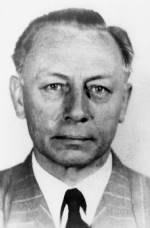
\includegraphics[width = \textwidth]{figures/wentzel}	
	\end{minipage}
	\begin{minipage}{0.315\textwidth}
	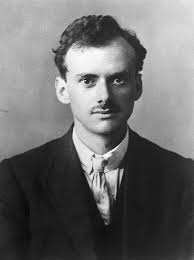
\includegraphics[width = \textwidth]{figures/dirac}	
	\end{minipage}
	\begin{minipage}{0.335\textwidth}
	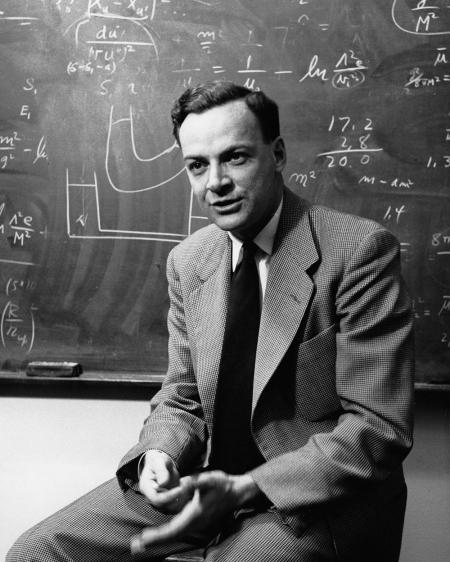
\includegraphics[width = \textwidth]{figures/feynman}	
	\end{minipage}
	
	\caption{Von links nach rechts: \\ \qquad \qquad \qquad \hspace{-3pt} G. Wentzel$\footnotemark$, P. A. M. Dirac$\footnotemark$ und R. P. Feynman$\footnotemark$}
\end{figure}
\footnotetext[1]{\tiny Quelle: https://research.uni-leipzig.de/catalogus-professorum-lipsiensium/leipzig/Wentzel\_378/}
\footnotetext[2]{\tiny Quelle: https://www.gettyimages.de/search/2/image?specificpeople=2032478\&sort=best }
\footnotetext[3]{\tiny Quelle: http://www.caltech.edu/news/feynmans-nobel-year-48524}
\end{frame}

\begin{frame}{Entwicklung des Formalismus}
	\begin{itemize}
		\item \textbf{1924: G. Wentzel} entdeckt 1924 das später nach Feynman benannte Pfadintegral. 
		\vfill 
		\item \textbf{1933: P. Dirac} erkennt die besondere Bedeutung des Wirkungsfunktionals für die klassische Mechanik, vgl. \cite{Dirac1934}.
		 \vfill 
		 \item \textbf{1948: R. Feynman} formuliert seine grundlegende, alternative Formulierung der Quantenmechanik, den Pfadintegral-Formalismus, vgl. \cite{Feynman1948}.
	\end{itemize}
\end{frame}